\documentclass[12pt]{iopart}
\usepackage{graphicx}
\usepackage[british,UKenglish,USenglish,american]{babel}
\usepackage[latin1]{inputenc}
\usepackage[T1]{fontenc}
\usepackage{latexsym}

\begin{document}
\title{Universal and morphological exponents for metabolic biological growth}
	\author{Felipe L. Pinheiro$^{1,}$, Andr\'{e} L. A. Penna$^2$, Fernando A. Oliveira$^{1,2}$}
	\address{
	$^1$ Instituto de F\'{i}sica, Universidade de Bras\'{i}lia, Brazil
}
	\address{
	$^2$ International Center for Condensed Matter Physics, Universidade de Bras\'{i}lia, Brazil
}
%\date{Received: date / Accepted: date}


%\maketitle

\begin{abstract}
In this work we investigated the biological growth exponents and we showed that they obey a combination of universal and empirical morphological exponents.  We applied these results for fishes and we obtained the exponents that describe their metabolic growth, and in addition we showed the influence of the exponents on the growth and the maturation time. We discuss the need to review some of the old empirical growth equations to give a better account of the data.\\
\noindent{\it Keywords\/} Universal exponent, Morphological exponent, Metabolic growth
\end{abstract}

\section{Introduction}
\label{intro}
The large diversity of forms and size of the living beings would at first glance induce us to believe that  no quantitative universal law could describe their behavior.  On the other  hand, since Darwin's evolution theory, we know that all living beings have a common origin and consequently we could expect common features underlying the basic mechanism. Based on that view, one could ask a question such as is there a universal law for growth? The last decades have seen a large number of  empirical evidence  and theoretical works that point towards two major simple rules:  First, a strict relationship between biological growth and  metabolic rates. Second, the existence of universal laws for metabolic rates, and consequently for the growth phenomena. Moreover, beyond the most optimistic expectation those laws are simple and universal.

The dependence of biological growth on the metabolic rates have been universally accepted. As such, it is common sense that the basal metabolic rate $B$ obeys an allotropic rate of the form \cite{Bertalanffy38a,Bertalanffy57,West97,West99,Brown05,Hatton15,Cebrian16,Rubner1883,Kleiber32,Banavar10,Agutter11}
\begin{equation}
B = b_0M^{\alpha},
\end{equation}
where $M$ is the mass of an average individual of a given species, $b_0$ is a constant and $\alpha$ is an exponent. However, more than a century was not enough to fix the  metabolic exponent $\alpha$.

In this work we call attention to the existence of universal and specific exponents in biological growth. In particular, we investigated the Bertalanffy equation \cite{Bertalanffy38a,Bertalanffy57}
\begin{equation}
L(t) = L_\infty \left[ 1 - e^{-(t+t_0)/\tau_\alpha} \right]\,,
\label{Ber}
\end{equation}
where $L(t)$ is the length as function of time, $\tau_\alpha$ is a growth time we shall discuss later, and $t_0$ is obtained by the animal size at birth. This equation has been used for decades and it is still used nowadays  in order to fit
the growth of fishes. We shall present here a generalization of this equation. Nevertheless this relationship has been used in many situations, and we shall show here that if we need a more precise fit of the available data we have to rewrite this equation into a more general form, see
Eq. (\ref{NBer}).

\section{Growth exponents}
In this section we come to the central point of this work, the relationship between the exponents.
Our starting point is that the growth mechanism is determined by the metabolic rate in such a way that the gain of mass at each time interval is due to major contributions: one which is proportional to the metabolic rate, which is the necessary energy to mass increment; the second term is the loss of matter that is proportional to the mass itself. Then it is given by
 \begin{equation}
\frac{dM}{dt} =c_1 M^{\alpha}-c_2 M\,,
\label{dM}
\end{equation}
where the second term on the right hand side  is a decay term which is proportional to the mass.
 This equation yields
\begin{equation}
M(t) = M_\infty \left[ 1 -(1-\epsilon_{\alpha}) e^{-t/\tau_\alpha} \right]^\delta\,,
\label{Mass}
\end{equation}
where
\begin{equation}
\epsilon_{\alpha} =  \chi^{\frac{1}{\delta}}\,.
\label{epsilon}
\end{equation}
Here $\chi=M_0/M_\infty$, with $M_0=M(0)$ as the initial mass, $M_\infty = M(\infty)=(c_1/c_2)^\delta$ as the saturation mass, and  $\delta = (1-\alpha)^{-1}$ as a universal exponent, because it depends only on $\alpha$ which is a universal parameter. Here
\begin{equation}
\label{tau}
\tau_{\alpha} =  \frac{\delta}{ c_1} M_\infty^{1/\delta}= \frac{\delta}{c_2}\,,
\end{equation}
is the average time of growth.   Although the expression $\chi$ could be extremely small,
$\epsilon_\alpha$ is not. For example for $\alpha=3/4$, $\delta=4$, a small $ \chi=0.01$, gives $\epsilon_{\alpha=3/4} \approx 0.32$,  which is a considerable amount compared with $1$. Consequently, it can not be neglected in Eq. (\ref{Mass}). However, there is  a "normal procedure" in the literature that consists of defining a time $t_0$ as in Eq. (\ref{Ber}) as $\exp(-t_0/\tau)=1-\epsilon_\alpha$. Even in the particular situation where we  consider $\epsilon_{\alpha}=0$, we can not consider  Eq (\ref{Ber}) as a good way to describe the growth phenomena, as we shall see below.

For the value of $\alpha$ we have two extreme views: The classical works of  Bertalanffy  \cite{Bertalanffy38a,Bertalanffy57}, which associates the metabolic rate to heat dissipation, being in this way proportional to the surface area
\begin{equation}
B \propto V^{2/3} \propto M^{2/3}.
\end{equation}
From these works it follows that $\alpha=2/3$. The works of West et al \cite{West97,West99,Brown05} attribute the metabolic rate to the energy necessary to feed each cell through the cardiovascular network. Their work suggest that the allotropic exponents should be multiples of $1/4$ and that $\alpha=3/4$. 

Recent results  show  that in macroecology the predator-prey power law biomass scales as well with $\alpha\approx 3/4$, which indicates that
very different communities of species exhibit similar high-level structure and function \cite{Hatton15,Cebrian16}. That conclusion was obtained through a massive amount of data for energy flows within the food chain for both terrestrial and aquatic biomes.

In table \ref{tab:alpha} we have the values of $\alpha$ given by several authors \cite{Kleiber32,Gano38,Brody45,Hayssen85,Elgar87,McNab88,Heusner91,Lovegrove00,Symonds02,White03,Savage04}, for more details see White and Seymours \cite{White05}. We note that for all the values but the second, we have $2/3 < \alpha < 3/4$. The empirical data  gives the average value for $\tilde{\alpha}$ = 0.72 $\pm$ 0.02 which if closer to $\alpha = 3/4$ than $\alpha = 2/3$.

The major exponents are connected, which give us important restriction for the growth exponents. First,
the relationship between the mass and the length is given by
\begin{equation}
M \propto L^\lambda,
\label{lamb}
\end{equation}
we shall call here $\lambda$  the morphological exponent.  Note that due the large diversity of forms we do not expect  $\lambda$  to be a universal exponent as $\alpha$ is. However, surprisingly it is remarkably close to $3$, see table 2.

 Fish growth is an important subject with scientific and practical applications \cite{Liu12,Katsanevakis08,Meinhardt07,Joshi12,Mateus07,Alejo-Plata11,Tang12,Matic-Skoko12,Sui12,Perez-Bote12,Clark99,Chabot16}.
 Now we will suppose that a fish has a  length $L(t)$  given by
 \begin{equation}
L(t) = L_{\infty} \left[  1 -(1-\epsilon_\alpha) e^{-t/\tau_\alpha}\right]^{\gamma}\,.
\label{NBer}
\end{equation}
Observe that it generalizes eq. (\ref{Ber}). To go beyond an empirical equation, we have to determine $\gamma$. Therefore, we consider  a lateral elliptical area, with  major axis $R_1(t)$,  and minor axis $R_2(t)$ given by 
\begin{equation}
R_i(t) = R_{i,\infty} \left[ 1 -(1-\epsilon_\alpha) e^{-t/\tau_\alpha} \right]^{\beta_i}\,,
%\label{eq:}
\end{equation}
with $i=1,2$. It is quite natural to consider the fish as  having a uniform and isotropic density, then we have
\begin{equation}
M \propto  R_1 R_2 L \propto  \left[1-(1-\epsilon_\alpha)e^{(-t/\tau_\alpha)}\right]^\delta\,,
%\label{}
\end{equation}
where
\begin{equation}
\delta =  2 \beta + \gamma\,,
\label{eq:par_1}
\end{equation}
where we consider $\beta = (\beta_1 + \beta_2)/2$ the average exponent for lateral growth. Since most of the data refer to $L(t)$,  we do not have  precise experimental information about the $R_i$. Consequently there is no reason to keep two $\beta_i$. For those with access to more detailed information we would suggest to obtain $\beta_1$,  $ \beta_2$ and to  check out the difference $\frac{|\beta_1 - \beta_2|}{2\beta}$, which we believe to be a small number. In any case,  it does not affect our analysis. Even for  the exponents $\beta$ and $\gamma$, we show here that there is not enough data to determine the difference between them.

From the relationship between Eq. (\ref{Mass}) and Eq. (\ref{lamb}) we get
\begin{equation}
\gamma = \frac{\delta }{\lambda}\,,
\label{eq:par_2}
\end{equation}
and
\begin{equation}
\beta = \frac{\delta}{2\lambda}(\lambda-1)\,.
\label{eq:par}
\end{equation}

\begin{table}%
\centering
\begin{tabular}{|c|c|c|c|c|c|c|c|c|c|c|c|c|}
\hline
$b_0$ & 2.6  & 1.8  & 2.3  & 4.3 &4.2 & 3.4 & 3.8 &4.1 &3.2 &4.0& 3.7 \\
$\alpha$  & 0.74  & 0.76  & 0.731  & 0.69  & 0.71  & 0.71  & 0.71 & 0.69  & 0.73  & 0.686  & 0.712  \\
Ref  &\cite{Kleiber32}  &\cite{Gano38} &\cite{Brody45}    &\cite{Hayssen85} &\cite{Elgar87} &\cite{McNab88} &\cite{Heusner91} &\cite{Lovegrove00} &\cite{Symonds02} &\cite{White03} &\cite{Savage04} \\
\hline
\end{tabular}
\caption{Basal metabolic rate, $B = b_0 M^\alpha$. All regressions were calculated to standardize units (BMR in ml~O$_2$~h$^{-1}$, M in g). The averages are $\tilde{\alpha}$ = 0.72 $\pm$ 0.02 and $\tilde{b_0}$ = 3.4 $\pm$ 0.7}
\label{tab:alpha}
\end{table}

\begin{table}%
\centering
\begin{tabular}{|c|c|c|c|}
\hline
Fish                                     & Ref                                                       & $\lambda$                     & $\tau_{2/3}$                  \\ \hline
Gymnosarda unicolor                      & ~~\cite{Joshi12}~~& ~~3.065~~ & ~~2.326~~ \\
pinirampus pirinampus                    & \cite{Mateus07}                        & 2.945                         & 3.333                         \\
pseudopaltystoma fasciatutum             & \cite{Mateus07}                        & 3.126                         & 7.692                         \\
Zungaro jahu                             & \cite{Mateus07}                        & 3.228                         & 7.813                         \\
pseudopaltystoma corruscans              & \cite{Mateus07}                        & 3.172                         & 7.874                         \\
dolphinfish Coryphaena hippurus (male)   & \cite{Alejo-Plata11}                   & 3.144                         & 0.977                         \\
dolphinfish Coryphaena hippurus (female) & \cite{Alejo-Plata11}                   & 2.848                         & 0.970                         \\
Protosalanx hyalocranius                 & \cite{Tang12}                          & 2.990                         & 0.341                         \\
oedalechlus labeo (male)                 & \cite{Matic-Skoko12}                   & 2.975                         & 7.463                         \\
oedalechlus labeo (female)               & \cite{Matic-Skoko12}                   & 3.014                         & 5.525                         \\
opsarrichthys bidens (male)              & \cite{Sui12}                           & 3.150                         & 3.226                         \\
opsarrichthys bidens (female)            & \cite{Sui12}                           & 3.050                         & 3.846                         \\
Sander Lucioperca                        & \cite{Perez-Bote12}                    & 3.010                         & 6.667                         \\ \hline
\end{tabular}
\caption{Parameters $\lambda$ and the growth time $\tau=\tau_{2/3}$ for each fish.  The average $\lambda$ is $\tilde{\lambda}$ = 3.06 $\pm$ 0.09.}
\label{tab1}
\end{table}  

Now we will analyze the relationship between our equation and the data existing in the literature, and we see that $\gamma= \beta=1$ only for $\lambda=\delta=3$ in discordance with the available data.

\begin{table}
\centering
\begin{tabular}{|c|c|c|c|}
\hline
$\alpha$        & $\delta$   & $\gamma$   & $\beta$    \\
\hline
$2/3$       & 3          & 1          & 1          \\
$3/4$       & 4          & 4/3          & 4/3        \\
0.72 $\pm$ 0.02 & 3.6 $\pm$ 0.1& 1.17 $\pm$ 0.05& 1.20 $\pm$ 0.05\\
\hline
\end{tabular}
\caption{Values of $\delta$, $\beta$ and $\gamma$  from the values of  $\alpha$. In the first two lines we use the expected value $\lambda=3$, in the last line we use the empirical $\lambda=3.06 \pm 0.09$.}
\label{tablegamma}
\end{table}

In Table 2 we show the values of the parameters for several species of fishes. There we display the empirical values of $\lambda$ and the growth time $\tau$ obtained using  Eq. (\ref{Ber}). Most of the authors treat the data with a  large number of decimals, however,   if we consider the standard deviation we see that the alleged accuracy is exaggerated and we have to look at those data with care. The major problem however lies in the many different ways to treat the data.

In table \ref{tablegamma} we obtain several exponents from the values of $\alpha$ and Eq. (\ref{eq:par_2}) and Eq.(\ref{eq:par}).   For the first and second line we take $\lambda=3$. For $\alpha=2/3$, Bertalanffy, we get $\delta=3$, and both
$\gamma=\beta=1$. For $\alpha=3/4$  we get $\delta=4$ and  $\gamma=\beta=4/3$.

From the empirical values $\alpha=0.72 \pm 0.02$ and $\lambda=3.06 \pm 0.09$  from table  \ref{tab1}, we get $\gamma=1.17 \pm 0.05$ and $\beta=1.20 \pm 0.05$.
From both second and third line  we note that both $\beta$ and $\gamma$ are always great than $1$, consequently the simple Bertalanffy equation, Eq. (\ref{Ber}), does not apply and if we want more precise information we need to use the more complete form Eq. (\ref{NBer}). Table \ref{tablegamma} shows as well a very small difference between the exponents $\beta$ and  $\gamma$.   Since  $\beta-\gamma \propto \lambda-3$,  and  $\lambda$ is very close to $3$, $\bar{\lambda} = 3.06 \pm 0.09$,  it is not surprising that we get the average values,  $\bar{\beta} \approx \bar{\gamma}$. Indeed, from the available data $\beta$ and $\gamma$ are very close, and for this particular issue more precise data are need to definitive conclusion. Thus, we can conclude that $\gamma \approx \beta > 1$, and we need to replace  Eq. (\ref{Ber}) by Eq. (\ref{NBer}).


\section{Growth Time}

The ratio between the two growth times is given by
\begin{equation}
\label{taurel}
\frac{\tau_{\alpha1}}{\tau_{\alpha2}}=\frac{c_{2}(\alpha_{2})}{c_{2}(\alpha_{1})}\left(\frac{1-\alpha_2}{1-\alpha_1}\right)\,.
\end{equation}
If we consider $c_2$ independent of $\alpha$ then, for example $\tau_{3/4}/\tau_{2/3}=4/3$. However, as we shall see below this naive argument does not apply, indeed both $c_{1}$ and $c_{2}$ must be strongly dependent on $\alpha$.

We now examine the relation between two growth times, for two different $\alpha$, in a more precise way. Since the total time evolution must be independent of $\alpha$, we define
\begin{equation}
	\eta=\frac{1}{\tau M_\infty^2}\int_0^{\infty}\left[M_{2/3}(t)-M_{\alpha}(t) \right]^2 dt\,,
\label{eq:eta}
\end{equation}
which must be minimized to reduce spurious differences. To avoid a cumbersome notation let us take $\tau=\tau_{2/3}$, $\epsilon = \epsilon_{2/3}=\chi^{1/3}$, such that $ \epsilon_{3/4}=\epsilon^{3/4}=\chi^{1/4}$.

For $\alpha=3/4$, we obtain

\begin{figure}%
\centering
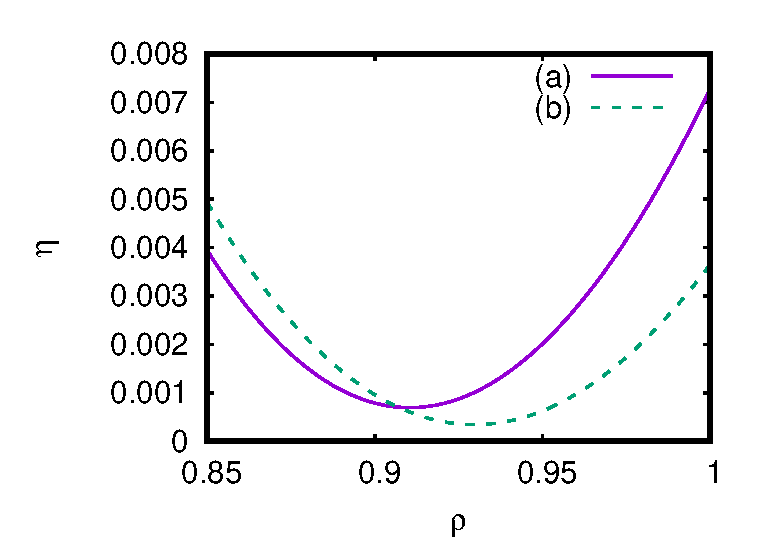
\includegraphics[width=.8\columnwidth]{figure_1}%figure_1
\caption{$\eta$ as a function of $\rho$. Curve (a) We use $\chi=M_0/M_\infty=10^{-3}$, which gives $\epsilon = 0.1$, we observe a minimum at $\rho*=0.91$ ; curve (b) $\chi=10^{-2}$, we have a minimum at $\rho*=0.93$.}
\label{fig:eta}
\end{figure}

\begin{figure}%
\centering
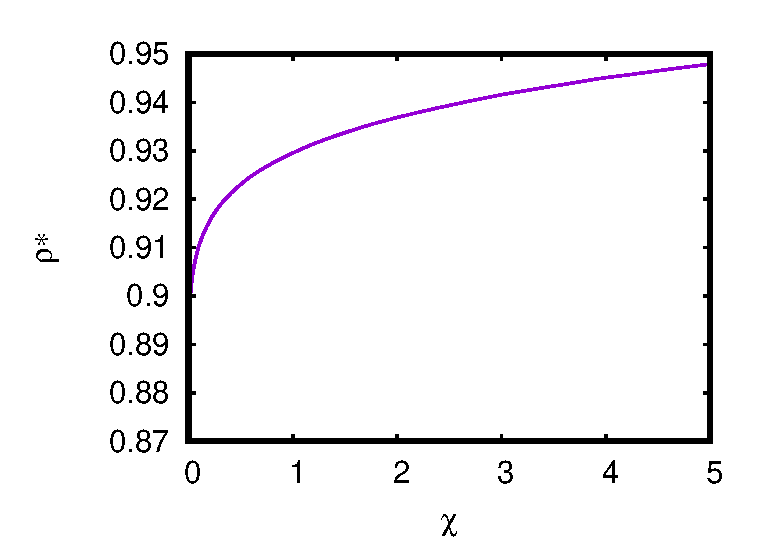
\includegraphics[width=.8\columnwidth]{figure_2}%figure_2
\caption{ The ratio between the growth times $\rho*$ as a function of the mass ratio $\chi=M_0/M_\infty$.  The $\chi$ axis is multiplied by $10^2$. }
\label{fig:rho}
\end{figure}


\begin{equation}
\eta  = f_1 + f_2 + g\,,
%\label{eq:}
\end{equation}
where $\rho=\tau_{3/4}/\tau_{2/3}$ and
\begin{eqnarray}
f_{1}&=&\sum_{i = 1}^3\sum_{j = 1}^3 \frac{A_{i}A_{j}}{i+j}\\
f_{2}&=&\rho\sum_{i = 1}^4\sum_{j = 1}^4 \frac{B_{i}B_{j}}{i+j}\\
g&=&-2\rho\sum_{i = 1}^3\sum_{j = 1}^4 \frac{A_{i}B_{j}}{i\rho+j}\,,
\end{eqnarray}
where $A_i=\left(\stackrel{3}{i}\right)(\epsilon -1)^{i}$ and $B_i=\left(\stackrel{4}{i}\right)(\epsilon^{3/4} -1)^{i}$. In this way, $\eta$ depends on the $\rho$ and $\epsilon$. For a given $\epsilon$, $\eta$ has a minimum $\frac{\partial \eta}{\partial \rho}=0$ for $\rho=\rho*$.

In  Fig. \ref{fig:eta} we plot $\eta$ as a function of $\rho$. There we see the ratio  $\chi=M_0/M_{\infty}$ influences the growth time, i.e., the minimum of $\eta$.  In curve (a), $\chi=M_0/M_{\infty}=10^{-3}$, which gives $\epsilon = 0.1$, with the minimum at $\rho*=0.91$; in curve (b) we have $\chi=10^{-2}$, which gives $\epsilon=0.215$, we see that now $\eta$ has a minimum of $\rho* = 0.93$. Since for fishes  $10^{-3} < \chi < 10^{-2}$ is a reasonable range for $\chi$, from that we can conclude that we have decreases in $\rho$ of less than of $10\%$, and not an increase as suggested by Eq. (\ref{taurel}).  In this way it becomes clear that the coefficients $c_1$ and $c_2$ are strongly dependent on the metabolic law, i.e on  $\alpha$.
It is very important to notice as well that a very small $\chi$ will demand a bit more of  growth time.

In Fig. \ref{fig:rho} we plot the value of $\rho*$, which minimizes $\eta$ as function of $\chi$.
Here, we multiply the $\chi$ axes by $10^{2}$.  The ratio $\rho*$ increases monotonically
as $\chi$ increases. In this way, we can say that fishes with small $\chi$ would have the growth
time more affected. However, this fraction is very small, i.e., an order of magnitude in $\chi$ will affect only $2\%$. Altogether, we can say that the growth time will be not affected by the metabolic exponent $\alpha$, neither by $\chi$. Consequently, the growth time is a very robust concept.

\section{Maturation time}

We now want to define the time parameter directly associated to reach the maturation mass according to its final mass. This maturation time can be known considering that the maturation mass finds the ideal value in $1-\exp{(-1)} \approx 63 \% $ of its maximum mass $M_{\infty}$. From Eq. (\ref{Mass}), the maturation time $\tau^*$ can be written as
\begin{equation}
\label{matu}
\tau^* =\frac{M(t)}{M_{\infty}}=\tau(\alpha) \ln{\left[\frac{1-\epsilon_{\alpha}}{1-(1-e^{-1})^{1-\alpha}}\right]}\,,
\end{equation}
where we have $\epsilon_{\alpha} \leq (1-e^{-1})^{1-\alpha}$.

In Fig. (\ref{fig:tau2}) we show $\tau^*$ as a function of $\chi$, for different values of $\alpha$. We take $\tau^*$ in units of $\tau(\alpha)$. We can see that both  curves decrease with $\chi$, but there are considerable numerical difference between them.
We see here a very large difference between the maturation time and the growth time, and how it is affected by the exponent $\alpha$.
This difference is higher than those observed in Figs. (1) and (2). Indeed, this is really something worth to observe in experiments.
\begin{figure}%
\centering
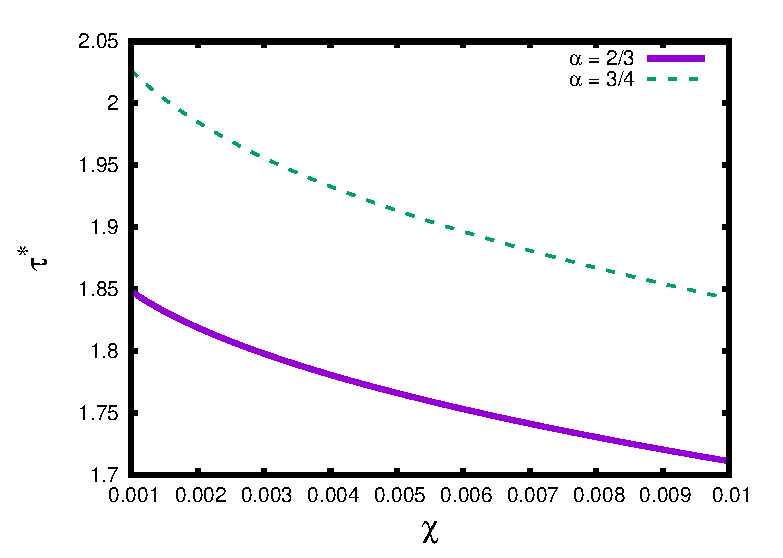
\includegraphics[width=.7\columnwidth]{figure_3}%figure_3
\caption{ $\tau^*$ as a function of $\chi$ for $\alpha = 3/4$, upper curve, and $\alpha = 2/3$, lower curve.}%
\label{fig:tau2}%
\end{figure}

\section{Conclusion}

In conclusion we have investigated the general  equations for growth in animals, starting from the basic metabolic rate that states that $B \propto M^{\alpha}$.  From this we determine that lateral growth exponent $\beta$ and the longitudinal growth exponent $\gamma$ as function of the the exponent $\delta$ and of the morphological exponent $\lambda$.  The morphological exponents $\beta$ and $\gamma$ are such that  $1 < \gamma \approx \beta \leq 4/3$. In any case the precision is enough to state that they are different from $1$ as exposed in Eq. (\ref{Ber}) and consequently the use of Eq. (\ref{NBer}) is necessary. We hope that new data could be used to verify the value of the exponents and in addition we expect that researchers  with experimental data could run it again using Eq. (\ref{NBer}) to validate the exponents. In addition to the exponents the major practical information coming from the analysis are the growth and maturation time, which are important in the laboratory, in fish farming, in fisheries, and for ecological modeling. We conclude that the growth time is very robust independent of the metabolic exponent. However, the maturation time is very sensible to rate $\chi=M(0)/M_{\infty}$ and $\alpha$.  Unfortunately, the  results existing in the literature come from different statistical methods used for treatment of the data, as well most of them do not state the measurement error.  Thus it is urgent to make this procedure more uniform.It would also be very important to see if the growth time is affected by stress such as in competition \cite{Barbosa17,Clerc10,Colombo12,Cunha09,Cunha11}.  A more sophisticated theory is necessary to take into account the influence of the temperature in the fish metabolism \cite{Clark99,Chabot16}. However, this goes beyond the objective of this work.

%\section{Acknowledgments}
\ack

We acknowledge the support of the Conselho Nacional de Desenvolvimento Cient\'{i}fico e Tecnol\'{o}gico (CNPq) Brazil, the Coordena\c{c}\~{a}o de Aperfei\c{c}oamento de Pessoal de N\'{i}vel Superior (CAPES) Brazil, and the Funda\c{c}\~{a}o de Apoio \`{a} Pesquisa do Distrito Federal (FAP-DF), Brazil.

%\bibliographystyle{jphysicsB}
\begin{thebibliography}{100}

\bibitem{Bertalanffy38a}{L.V. Bertalanffy}, {A quantitative Theory of orgonic Growth}, \textit{Hum. Biol.}, \textbf{10}, {181} {(1938)}.

\bibitem{Bertalanffy57}{L.V. Bertalanffy}, {Quantitative laws in metabolism and growth}, \textit{Q. Rev. Biol.}, \textbf{32}, {217} {(1957)}.

\bibitem{West97}{G.B. West }, {A General Model for the Origin of Allometric Scaling Laws in Biology}, \textit{Science}, \textbf{276}, {122} {(1997)} .

\bibitem{West99}{ G.B. West, J.H. Brown, and B.J. Enquist}, { The origin of universal scaling laws in biology}, \textit{Physica A}, \textbf{263}, {104} {(1999)}.

\bibitem{Brown05}{J.H. Brown, G.B. West, and B.J. Enquist}, {Yes, West, Brown and Enquist's model of allometric scaling is both mathematically correct and biologically relevant}, \textit{Funct. Ecol.}, \textbf{19}, 735 {(2005)}.

\bibitem{Hatton15}{ I.A. Hatton, K.S. McCann, J.M. Fryxell, et al.}, {The predator-prey power law: Biomass scaling across terrestrial and aquatic biomes}, \textit{Science}, \textbf{349}, {1070} {(2015)}.

\bibitem{Cebrian16}{J. Cebrian}, {Energy flows in ecosystems}, \textit{Science}, \textbf{349},  {1053} {(2015)}.

\bibitem{Rubner1883} M. Rubner, {{\"{U}}ber den einfluss der k{\"{o}}rpergr{\"{o}}sse auf stoff- und kraftwechsel}, \textit{Z. Biol.}, \textbf{19},  536 (1883).

\bibitem{Kleiber32} M. Kleiber, {Body size and metabolism}, \textit{Hilgardia}, \textbf{6}, 315 (1932).

\bibitem{Banavar10}{J.R. Banavar, M.E. Moses, J.H. Brown, J. Damuth, A. Rinaldo, R.M. Sibly, and A. Maritan}, {A general basis for quarter-power scaling in animals}, \textit{Proc. Natl. Acad. Sci.}, \textbf{107}, {15816} {(2010)}.

\bibitem{Agutter11}{P.S. Agutter and J.A. Tuszynski}, {Analytic theories of allometric scaling}, \textit{J. Exp. Biol.}, \textbf{214}, 1055 {(2011)}.

\bibitem{Gano38} {F. Gano}, {Vital energetics : a study in comparative basal metabolism}. {Washington, D.C. : Carnegie Institution of Washington}, {(1938)}.

\bibitem{Brody45} S. Brody, {Bioenergetics and growth: with special reference to the efficiency complex in domestic animals.}. A Publication of the Herman Frasch Foundation, Reinhold Publishing Corp., New York, (1945).

\bibitem{Hayssen85} V. Hayssen and R.C. Lacy, {Review basal metabolic rates in mammals:  taxonomic differences in the allometry of BMR and body mass}, \textit{Comp. Biochem Physiol}, \textbf{81A},  741 (1985).

\bibitem{Elgar87} M.~A. Elgar and P.H. Harvey, {Basal Metabolic Rates in Mammals: Allometry, Phylogeny and Ecology}, \textit{Funct. Ecol.}, \textbf{1}, 25 (1987).

\bibitem{McNab88} B.~K. McNab, {Complications inherent in scaling the basal rate of metabolism in mammals}, \textit{The Quarterly Review of Biology}, \textbf{63}, 25 (1988).

\bibitem{Heusner91} A.A~Heusner, {Size and power in mammals}, \textit{ J. Exp. Biol.}, \textbf{54}, 25 (1991).

\bibitem{Lovegrove00} B.G.~Lovegrove, {The Zoogeography of Mammalian Basal Metabolic Rate.}, \textit{Am. Nat.}, \textbf{156}, 201 (2000).

\bibitem{Symonds02} M.R.E. Symonds and M.~a Elgar, {Phylogeny affects estimation of metabolic scaling in mammals}, \textit{Evolution}, \textbf{56}, 2330 (2002).

\bibitem{White03} C.R. White and R.S. Seymour, {Mammalian basal metabolic rate is proportional to body mass $2/3$}, \textit{PNAS}, \textbf{100}(7), 4046 (2003).

\bibitem{Savage04} V.M.~Savage and JF~Gillooly, {The predominance of quarter-power scaling in biology}, \textit{Funct. Ecol.}, \textbf{18}, 257 (2004).

\bibitem{White05}{C.R. White and R.S. Seymour }, {Allometric scaling of mammalian metabolism}, \textit{J. Exp. Biol.}, \textbf{208}, {1611} {(2005)}.

\bibitem{Liu12}{Q. Liu, B. Xu, Z. Ye, and Y. Ren }, {Growth and mortality of small yellow croaker (Larimichthys polyactis) inhabiting Haizhou bay of China}, \textit{J. Ocean Univ. China}, \textbf{11}, {557} {(2012)}.

\bibitem{Katsanevakis08}{S. Katsanevakis and C.D. Maravelias}, {Modelling fish growth: multi-model inference as a better alternative to a priori using von Bertalanffy equation}, \textit{Fish Fish.}, \textbf{9}, {178} {(2008)}

\bibitem{Meinhardt07}{H. Meinhardt, A.F. Quadros, and P.B. Araujo}, {Growth curve of Balloniscus glaber Araujo \& Zardo (Crustacea, Isopoda, Oniscidea) from Parque Estadual de Itapu\~{a}, Rio Grande do Sul, Brazil}, \textit{Rev. Bras. Zool. }, \textbf{24}, {1108} {(2007)}.

\bibitem{Joshi12}{ K.K. Joshi}, {Fishery, biology and dynamics of dogtooth tuna, Gymnosarda unicolor (R\"{u}ppell, 1838) exploited from Indian seas}, \textit{Indian J. Fish.}, \textbf{59}, {75} {(2012)}.

\bibitem{Mateus07}{L.A.F. Mateus and J.M.F. Penha }, {Din\^{a}minca poulacional de quatro esp\'{e}cies de grandes bagres na bacia do rio Cuiab\'{a}, Pantanal norte, Brasil (siluriformes, Pimelodidae)}, \textit{ Rev. Bras. Zool.}, \textbf{24}, 87 {(2007)}.

\bibitem{Alejo-Plata11}{C. Alejo-Plata }, {Edad y crecimiento del dorado Coryphaena hippurus, en el Golfo de Tehuantepec, M\'{e}xico}, \textit{Rev. Biol.}, \textbf{46}, 125 {(2011)}.

\bibitem{Tang12}{F.J. Tang, W. Liu, J. Wang, R. Froese, and S. Xie}, {Growth, length-weight relationship and biological information on the clearhead icefish (Protosalanx hyalocranius Abbott, 1901) in Lake Khanka (Xingkai)}, \textit{J. Appl. Ichthyol.}, \textbf{28}, 842 {(2012)}.

\bibitem{Matic-Skoko12}{S. Mati{\'{c}}-Skoko, J. Ferri, M. Kraljevi{\'{c}}, and A. Pallaoro }, {Age estimation and specific growth pattern of boxlip mullet, Oedalechilus labeo (Cuvier, 1829) (Osteichthyes, Mugilidae), in the eastern Adriatic Sea}, \textit{J. Appl. Ichthyol.}, \textbf{28}, 182 (2012).

\bibitem{Sui12}{ XY~Sui, YZ~Yan, and YF~Chen}, {Age, Growth, and Reproduction of Opsariichthys bidens (Cyprinidae) from the Qingyi River at Huangshan Mountain, China}, \textit{Zool. Stud.}, \textbf{51}, 476 {(2012)}.

\bibitem{Perez-Bote12}{J.L. P{\'{e}}rez-Bote and R. Roso }, {Growth and length-weight relationships of Sander lucioperca (Linnaeus, 1758) in the Alc{\'{a}ntara Reservoir, south-western Spain: comparison with other water bodies in Eurasia}, \textit{J. Appl. Ichthyol. }, \textbf{28}, 264 {(2012)}.

\bibitem{Barbosa17}{F. V. Barbosa, A. L. A.  Penna, R. M. S. Ferreira, K. L. V. Novais, J. A.R. da Cunha, F. A. Oliveira}, {Pattern transitions and complexity for a nonlocal logistic map}, \textit{Physica A}, \textbf{473}, {301} {(2017)}.

\bibitem{Clerc10}{M. G. Clerc, D. Escaff and V. M. Kenkre}, {Analytical studies of fronts, colonies, and patterns: Combination of the Allee effect and nonlocal competition interactions}, \textit{Phys. Rev. E}, \textbf{82}, {036210} {(2010)}.

\bibitem{Colombo12} {E.H. Colombo and C. Anteneodo}, {Nonlinear diffusion effects on biological population spatial patterns},  \textit{Phy. Rev. E}, \textbf{86}, 036215 (2012). 

\bibitem{Cunha09} {J.A.R. da Cunha, A.L.A. Penna, M.H. Vainstein, R. Morgado, and F.A. Oliveira}, {Self-organization analysis for a nonlocal convective Fisher equation}, \textit{Phys. Lett. A}, \textbf{373}, 661 {(2009)}.

\bibitem{Cunha11} {J.A.R. da Cunha, A.L.A. Penna, and F.A. Oliveira}, {Pattern formation and coexistence domains for a nonlocal population dynamics}, \textit{Phys. Rev. E}, \textbf{83}, {R015201} {(2011)}.

\bibitem{Clark99} { A. Clarke and  N. M. Johnston}, {Scaling of metabolic rate with body mass and temperature in teleost fish}, \textit{Journal of animal ecology}, \textbf{68},  893-905 (1999).}

\bibitem{Chabot16} {D. Chabot , J. F. Steffesen and A. P. Farrell}, {The determination of standard metabolic rate in fishes}, \textit{Journal of Fish Biology}, \textbf{88} , 81-121 (2016).

\end{thebibliography}

\end{document}

